
\chapter{Software Architektur}
\section{Anforderungen}
\label{sec:Anforderungen} 
%Christoph

Im Folgenden sollen die Anforderungen an die Studienarbeit festgelegt werden. \newline
Ein Hauptbestandteil der Arbeit besteht darin, ein Vorgängerprojekt mit einer AR.Drone 2.0 in das ROS Framework zu portieren.
Dies beinhaltet eine Modularisierung der Projektbestandteile in ROS Nodes. Ziel soll sein, den Quadrocopter mit Hilfe einer Kinect und Gestenerkennung steuern zu können. Anzumerken ist, dass ROS nur unter UNIX basierten Betriebssystemen läuft und das bestehende Projekt Libraries verwendet, welche nur unter Windows verfügbar sind. \newline
Eine weitere Vorgabe besteht darin, dass man neben der realen Drohne jegliche Funktionalität auch in einer Simulation laufen soll. \newline
Somit kann man für Präsentationen, in denen der Flug einer Drohne nicht möglich ist, den Quadrocopter in einer frei gestaltbaren simulierten Umgebung fliegen lassen. \newline
Ein weiterer Bestandteil dieser Arbeit besteht darin, Ansätze und Limitationen der Implementierung eines Assistenzsystems zu testen und zu bewerten. Dafür soll ein externes Projekt, zur Gewinnung von Tiefenbildern aus einer monokularen Kamera, in die Projektumgebung integriert werden. Hierbei soll es wiederum möglich sein, dass die Videostream sowohl von der realen, als auch von der simulierten Drohne gesendet werden kann. \newline
Es soll dabei ermittelt werden, ob die Nutzung der Software für den Anwendungszweck praktikabel und sinnvoll ist.

%hier weitermachen, wenn man weiß wie weit wir tatsächlich kommen #wahrscheinlichsindwirzublöd #forschung>implementierung

%	-> Wände / Türen erkennen
%	-> aktives eingreifen der Drohne in das Geschehen -> Kollisionsvermeidung


\section{Überblick}
\label{Überblick}

\section{Bildverarbeitung}
\label{Bildverarbeitung}
In diesem Abschnitt wird beschrieben, wie Drohne aus den Bildern der Kamera Informationen gewinnen kann, die später für die Betrachtung des Assistenzsystems relevant sind. 
%-> errechnung von bewegungen + tiefenbildanalyse
%basierend auf paper Christian Forster, Matia Pizzoli, Davide Scaramuzza
%In diesem Abschnitt soll die technische Ausführung beschrieben werden.

\subsection{Semi-Direct Monocular Visual Odometry - SVO}


Eine Grundanforderung an das Projekt ist die Nutzung einer nicht modifizierten AR.Drone. Dadurch entsteht die Problematik, dass man keine Tiefenbildkamera nutzen kann, um in Echtzeit Tiefenbilder zu generieren. Die Drohne ist lediglich mit einer monokularen \footnote{Monokular ist die Bezeichnung für Kameras mit einer einzelnen Linse} Frontkamera ausgestattet. \newline
Um Tiefeinformationen aus den Bildern einer solchen Kamera zu gewinnen, wird eine Szene aus verschiedenen Perspektiven aufgenommen. Anschließend gibt es unterschiedliche Ansätze um aus den aufeinanderfolgenden Bildern Kamerapositionen und Umgebungsstrukturen zu ermitteln. \newline
Der aktuelle Standard sind Feature basierte Methoden. Diese versuchen die wichtigsten Merkmale eines Bildes, die Features, zu extrahieren. Mit Hilfe von Feature Deskriptor Algorithmen werden Vektoren mit Informationen zu invarianten Features berechnet, welche als Fingerabdruck für diese Merkmale fungiert. \newline
Aufeinanderfolgende Bilder werden dann mit Hilfe dieser Feature Deskriptoren abgeglichen und sowohl Kamerabewegungen, als auch Strukturen werden rekonstruiert. Zur Optimierung sind abschließend die ermittelten Kamerapositionen anzugleichen. Dies geschieht mit Hilfe von Algorithmen zur Minimierung des Reprojektionsfehlers. \footnote{Reprojektionsfehler sind geometrische Fehler die im Zusammenhang zwischen abgebildeten und berechneten Bildpunkten entstehen.} 
\newline
%\cite{} https://en.wikipedia.org/wiki/Reprojection_error
%Bilder dazu hier einfügen
Ein weiterer Ansatz ist die direkte Methode. Hierbei werden die Features nicht über Deskriptor Algorithmen bestimmt, sondern das Problem wird über die Intensitäten der Pixel gelöst. Bei einem Graustufenbild kann entspricht diese Intensität der Helligkeit von Bildbereichen. \newline
Somit kann bei der Rekonstruktion im Gegensatz zum Feature basierten Ansatz auch die Richtung der Gradienten von Intensitäten genutzt werden. Dadurch funktioniert diese Methode auch bei Bildern mit sehr wenig Textur, Bewegungsunschärfe und fehlerhaftem Kamerafokus. \newline
Das für diese Arbeit relevante Vorgehen kombiniert die Vorteile der beschriebenen Methoden. Die Semi direkte Odometrie %footnote dazu
verwendet einen Algorithmus der ebenfalls auf Feature Zusammenhängen basiert. Diese werden jedoch implizit direkten Bewegungsabschätzung bezogen, anstatt explizit durch Algorithmen mit Feature Deskriptoren berechnet zu werden. \newline
Dadurch müssen Features nur extrahiert werden, wenn diese noch nicht auf einem der vorherigen Bildern vorhanden war. Insgesamt ist dieser Ansatz somit schnell, da wenig Berechnungen pro Bild stattfinden und auf Grund Verwendung der Intensitätsgradienten sehr genau und robust. \newline
Diese Eigenschaften sind für die Anforderungen der Studienarbeit essentiell, da die Drohne sich sehr schnell bewegen kann und somit in möglichst kurzer Zeit neue Bilder auswerten muss. Das beschrieben Verfahren minimiert damit die Auswirkungen der typischen Probleme von Drohnen. Diese sind vorwiegend die niedrige Texturierung, welche in Innenräumen auftreten kann, sowie kameraspezifische Probleme wie Bewegungsunschärfe und der Verlust des Kamerafokus.


\subsection{Regularized Monocular Depth Estimation - REMODE}



\subsection{Kamerakalibrierung}
Ein Grundproblem der Bildverarbeitung ist die Verzerrung des Bildes. Da aus eingehenden Bildern Features erkannt werden sollen und aus diesen darüber hinaus Abstände berechnet werden, ist es essentiell, dass die Kamera richtig kalibriert ist. \newline
Hierbei unterstützt SVO drei Kamera Modelle: ATAN, Pinhole und Ocam. \cite{svo_cameracalibration} \newline
Das ATAN Model basiert auf dem \textit{Field of View \emph{(FOV)}} Verzerrungsmodell. 



\section{Bildverarbeitung}
\label{Bildverarbeitung}

\subsection{Featureerkennung}
\subsection{Kinect}
%Max
\subsection{Die einzelnen ROS Nodes}
%Beide
\subsection{Architektur}
%Beide



%Bild der Drohne http://lightspots.ch/images/ARdronebw.png
%Bild vom Typ https://img.clipartfox.com/d02b01c31b79dd51b6c2c6a2a5db5985_stop-help-vector-art-outstretched-arm-clipart_416-416.jpeg
%Bild von kinect https://d3nevzfk7ii3be.cloudfront.net/igi/DtuTZhDHRWaOirBm.large
%\begin{figure}[ht]
%	\centering
%	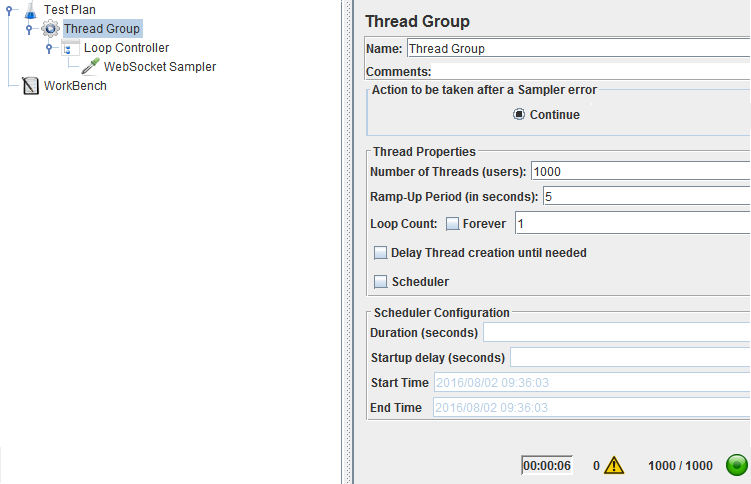
\includegraphics[scale=0.7]{Bilder/jMeterReal.png}
%	\caption[Testing with jMeter]{jMeter testing}
% 	\label{fig:testing}
%\end{figure}


